\section{Classement proprioceptif}

\subsection{Classement proprioceptif}    
    \begin{frame}
        \frametitle{Classement proprioceptif}
        Le classificateur proprioceptif est indépendant du classificateur
        extéroceptif. \\ \vspace{5mm}
        Deux classificateur proposés :
        \begin{itemize}
            \item basée sur les vibrations ;
            \item basée sur la force de traction.
        \end{itemize}
          
    \end{frame}
    
\subsection{Première approche}    
    \begin{frame}
        \frametitle{Première approche}
        \begin{itemize}
            \item Les terrains mécaniquement différents induisent différentes vibrations.
            \item Approche développée par Brooks (2004) et Brook et Iagnemma (2005).
            \item Amélioration par utilisation de \textit{Support Vector Machine} (SVM) pour la classification.
        \end{itemize}          
    \end{frame}
    
    \begin{frame}
        \frametitle{Validation expérimentale (robot)}
        \begin{columns}[c]
            \begin{column}{0.5\textwidth}
                \begin{figure}
                    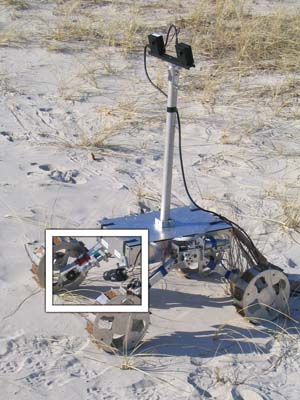
\includegraphics[height=0.6\textheight]{./media/tortoise.jpg}
                    \captionsetup{justification=centering}                         
                    \caption{Robot TORTOISE}
                \end{figure}
            \end{column}
            
            \begin{column}{0.5\textwidth}
                \begin{figure}
                    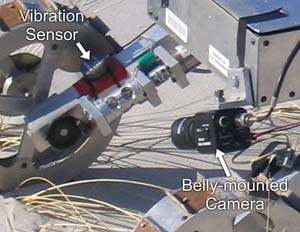
\includegraphics[width=\textwidth]{./media/vibrationSensor.jpg}
                    \captionsetup{justification=centering}
                    \caption{Capteur de vibrations}
                    \note{Microphone directement sur la suspension avant droite et enregistrement via l'entré audio de l'ordi}
                    \note{Importance du robot dans les expériences}
                \end{figure}
            \end{column}
        \end{columns}            
    \end{frame}
    
    \begin{frame}
        \frametitle{Validation expérimentale (environnement)}
        \begin{figure}
            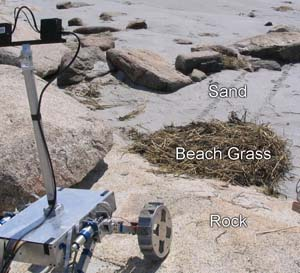
\includegraphics[height=0.6\textheight]{./media/beach.jpg}
            \caption{Plage de Wingaersheek}
            \note{Beach grass ajouté pour démontrer l'efficacité en multiclasses}
            \note{Étiquette pour les vibrations attribués manuellement}
        \end{figure}
    \end{frame}

    \begin{frame}
        \frametitle{Résultats}
        Comparaison des vrais positifs (VP) par rapport au faux positifs (FP) :\\
        \begin{center}              
            \begin{tabular}{|lcc|}
                \hline
                Classe & VP (\%) &  FP (\%)\\
                \hline
                Roche & > 50 & < 1 \\
                Herbes & > 50 & < 3 \\
                Sable & > 50 & < 5\\
                \hline           
            \end{tabular}        
        \end{center} 
        Confiance de l'étiquettes de classe attribué à un terrain : 92,3\%.
    \end{frame}
    
\subsection{Deuxième approche}
    \begin{frame}[allowframebreaks]
        \frametitle{Deuxième approche}
        \begin{itemize}
            \item Basé sur la force de traction net entre la roue et le sol.
            \item Données utilisées :
            \begin{itemize}
                \item couple (torque) : courant moteur ou capteur dédié ;
                \item enlisement : camera ou capteur dédié.
            \end{itemize}
            \item Métrique de traversabilité : coefficient de traction ($\mu_{tr}$) définie par Wong (2001).            
            \item Prédiction des bornes inférieures et supérieures de $\mu_{tr}$ et classement suivant les bornes inférieures
            \note{Haut risque = classement conservateur}
            \note{Borne déterminé avec algo d'optimisation numérique (modèle Bekker sans solution)}
        \end{itemize}
        
    \end{frame}
    
    \begin{frame}
        \frametitle{Validation expérimentale (banc d'essai)}
        \begin{columns}
            \begin{column}{0.5\textwidth}
                \vspace{-3mm}
                \begin{figure}
                    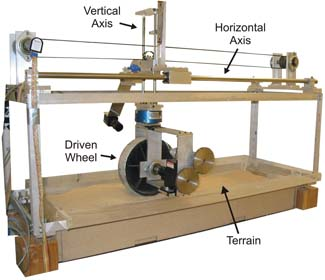
\includegraphics[width=0.8\textwidth]{./media/testBed.jpg}
                    \captionsetup{justification=centering}
                    \caption{Banc d'essai d'interaction roue-sol}
                    \note{Env. contrôlé, traverse a vitesse constante le bac, 5 type de surface, contrôle vitesse/vitesseAngulaire séparément}
                \end{figure}
            \end{column}         
            
            \begin{column}{0.5\textwidth}
                \begin{figure}
                    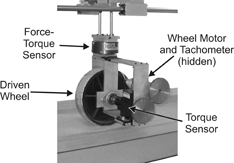
\includegraphics[width=0.8\textwidth]{./media/testBedSensors.png}
                    \captionsetup{justification=centering}
                    \caption{Appareils de mesure}
                \end{figure}
            \end{column}
        \end{columns}        
    \end{frame}
    
    \begin{frame}
        \frametitle{Validation expérimentale (Wingaersheek)}
        \begin{itemize}
            \item Couple mesuré avec un capteur dédié.
            \item Enlisement mesuré avec une caméra selon l'approche proposé par Brooks et al. (2006)
            \item Mesures effectuées sur la roue avant droite.
            \begin{itemize}
                \item Le cotrôle de la vitesse du robot est approximativement égale à la vitesse des trois autres roues. 
            \end{itemize}
            \item Valeurs de référence établies avec la caméra
        \end{itemize}
    \end{frame}    
    
    \begin{frame}
        \frametitle{Résultats de validation (banc d'essai)}
        \begin{figure}
            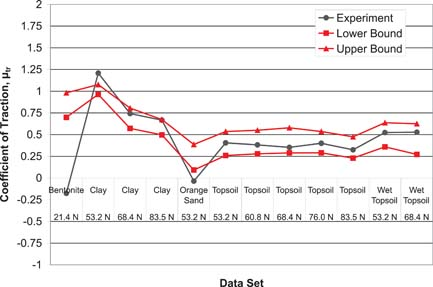
\includegraphics[width=0.7\textwidth]{./media/tractionResults.jpg}
            \captionsetup{justification=centering}
            \caption{Résultats d'estimation de la traction en banc d'essai}
            \note{Décrire les axes, différent data/force, expliquer 3 outliers -> le modèle ne représente pas bien les distributions de stress pour les mu <0 et >1}
            \note{Valeur médiane de torque et d'enlisement utilisés pour chaque run p.455 top left}
            \note{Analyse des différents terrains, vertical load et wheel slip}
        \end{figure}         
    \end{frame} 
    
    \begin{frame}
        \frametitle{Résultats de validation (Wingaersheek)}
        \begin{columns}[c]
            \begin{column}{0.5\textwidth}
                \begin{figure}
                    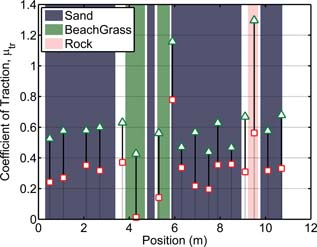
\includegraphics[width=0.9\textwidth]{./media/beachTraction.jpg}
                    \captionsetup{justification=centering}
                    \caption{Résultats d'estimation de la traction}
                \end{figure}                                
            \end{column}
            \small
            \begin{column}{0.5\textwidth}
                \vspace{-11mm}
                \begin{figure}  
                \begin{tabular}{lc}
                    \hline
                    Classe & Intervalle pour la \\&borne inférieur de $\mu_{tr}$ \\
                    \hline
                    A & 0,5 à $\infty$\\
                    B & 0,25 à 0,5\\
                    C & 0,1 à 0,25\\
                    D & 0 à 0,1\\
                    E & $-\infty$ à 0\\
                    \hline           
                \end{tabular}
                \captionsetup{justification=centering}
                \caption{Étiquettes des classes pour $\mu_{tr}$}
                \end{figure}
                \note{La discrétisation est nécessaire au framework self-sup.}   
            \end{column}
        \end{columns}
    \end{frame}       
    